\RequirePackage{ifluatex}
\documentclass[ngerman,a4paper]{report}
%\usepackage[top=2cm,bottom=2cm,left=1cm,right=1cm]{geometry}
\usepackage[ngerman]{babel}
%\usepackage[utf8]{inputenc} %not recommended with lualatex

\usepackage{zref-base}
\usepackage{etoolbox}
\usepackage{xparse}%better macros
\usepackage{chngcntr}
\usepackage{calc}

\usepackage[T1]{fontenc}
\ifluatex
\usepackage{fontspec}
\fi

\usepackage[texindy]{imakeidx}
\makeindex[name=semester1,title={Symbolverzeichnis (1. Semester)}]
\makeindex[name=semester2,title={Symbolverzeichnis (2. Semester)}]
\makeindex[name=symbols,title=Symbolverzeichnis]

\usepackage[xindy,acronym]{glossaries}
\makeglossaries

\usepackage{amsmath}
\usepackage{amssymb}
\usepackage{amsfonts}
\usepackage{mathtools}
\usepackage{latexsym}
\usepackage{marvosym} %lighning
\usepackage{bbm} %unitary matrix 1
\usepackage{cancel}
\usepackage{xfrac}%sfrac -> fractions e.g. 3/4

\usepackage[table]{xcolor}
\usepackage{graphicx}

\usepackage{enumerate}
\usepackage{enumitem} %customize label

\usepackage{tabularx}
\usepackage{multirow}
\usepackage{booktabs}

\usepackage{ulem} %better underlines

\usepackage{parskip}%split paragraphs by vspace instead of intendations
\usepackage{tocloft}
\usepackage{fancyhdr}
\usepackage{titlesec}%customize titles
\usepackage{marginnote}

\usepackage[amsthm,thmmarks,hyperref]{ntheorem}%customize theorem-environments more effectively
\usepackage[ntheorem,framemethod=TikZ]{mdframed}

\usepackage[bookmarks=true]{hyperref}
\hypersetup{
	colorlinks,
	citecolor=green,
	filecolor=green,
	linkcolor=blue,
	urlcolor=green
}
\usepackage{cleveref}
\usepackage{bookmark}

\newcommand{\coloredRule}[3][black]{\textcolor{#1}{\rule{#2}{#3}}}
\newlength{\blacktrianglewidth}
\settowidth{\blacktrianglewidth}{$\blacktriangleright$}

\definecolor{lightgrey}{gray}{0.91}
\definecolor{lightred}{rgb}{1,0.6,0.6}
\definecolor{darkgrey}{gray}{0.6}
\definecolor{darkgreen}{rgb}{0,0.6,0}

%numbered theorems
\theoremstyle{break}
\theorembodyfont{}

\mdfdefinestyle{boxedtheorem}{%
	outerlinewidth=3pt,%
	skipabove=5pt,%
	skipbelow=10pt,%
	frametitlefont=\normalfont\bfseries\color{black},%
}

\newmdtheoremenv[%
style=boxedtheorem,%
innertopmargin=\topskip,%
innerbottommargin=\topskip,%
linecolor=darkgrey,%
backgroundcolor=lightgrey,%
]{theorem}{Theorem}[section]
\newmdtheoremenv[%
style=boxedtheorem,%
linecolor=darkgrey,%
topline=false,%
rightline=false,%
bottomline=false,%
innertopmargin=\topskip,%
innerbottommargin=\topskip,%
backgroundcolor=lightgrey,%
]{proposition}[theorem]{Satz}
\newmdtheoremenv[%
style=boxedtheorem,%
linecolor=darkgrey,%
topline=false,%
rightline=false,%
bottomline=false,%
backgroundcolor=lightgrey,%
innertopmargin=\topskip,%
innerbottommargin=\topskip,%
]{lemma}[theorem]{Lemma}
\newmdtheoremenv[%
style=boxedtheorem,%
linecolor=red,%
topline=false,%
rightline=false,%
bottomline=false,%
innertopmargin=0,%
innerbottommargin=-3pt,%
]{definition}[theorem]{Definition}
\newmdtheoremenv[%
outerlinewidth=3pt,%
linecolor=black,%
topline=false,%
rightline=false,%
bottomline=false,%
innertopmargin=0pt,%
innerbottommargin=-3pt,%
frametitlefont=\normalfont\bfseries\color{black},%
skipabove=5pt,%
skipbelow=10pt,%
]{conclusion}[theorem]{Folgerung}
\newmdtheoremenv[%
hidealllines=true,%
frametitlefont=\normalfont\bfseries\color{black},%
innerleftmargin=0pt,%
skipabove=5pt,%
innerleftmargin=10pt,%
]{remark}[theorem]{\hspace*{-10pt}$\blacktriangleright$\hspace*{\dimexpr 10pt - \blacktrianglewidth\relax}Bemerkung}
\newmdtheoremenv[%
hidealllines=true,%
frametitlefont=\normalfont\bfseries\color{black},%
innerleftmargin=10pt,%
]{example}[theorem]{\hspace*{-10pt}\rule{5pt}{5pt}\hspace*{5pt}Beispiel}

%unnumbered theorems
\theoremstyle{nonumberbreak}
\theoremindent0cm
\newmdtheoremenv[%
style=boxedtheorem,%
linecolor=red,%
topline=false,%
rightline=false,%
bottomline=false,%
innertopmargin=0,%
innerbottommargin=0pt,%
]{*definition}{Definition}
\newmdtheoremenv[%
hidealllines=true,%
frametitlefont=\normalfont\bfseries\color{black},%
innerleftmargin=0pt,%
skipabove=5pt,%
innerleftmargin=10pt,%
]{*remark}{\hspace*{-10pt}$\blacktriangleright$\hspace*{\dimexpr 10pt - \blacktrianglewidth\relax}Bemerkung}
\newmdtheoremenv[%
hidealllines=true,%
innerleftmargin=10pt,%
]{*example}{\hspace*{-10pt}\rule{5pt}{5pt}\hspace*{5pt}Beispiel}

%Hinweis-Theoremstyle and environment
%To get rid of the parentheses, a new theorem style is neccessary (definition of nonumberbreak from ntheorem.sty)
%to achieve the underlining, this needed to put in the theoremstyle definition
\theoremheaderfont{\mdseries}
\theoremseparator{:}
\theorempostskip{0pt}
\makeatletter
\newtheoremstyle{noparentheses}%
	{\item[\rlap{\vbox{\hbox{\hskip\labelsep \theorem@headerfont
					\uline{##1}\theorem@separator}\hbox{\strut}}}]}%
	{\item[\rlap{\vbox{\hbox{\hskip\labelsep \theorem@headerfont
					\uline{##1\ ##3\theorem@separator}}\hbox{\strut}}}]}
\newtheoremstyle{underlinedPlain}%
	{\item[\hskip\labelsep \uline{\theorem@headerfont ##1\theorem@separator}]}%
	{\item[\hskip\labelsep \uline{\theorem@headerfont ##1\ (##3)\theorem@separator}]}
\makeatother

\theoremstyle{noparentheses}
\newmdtheoremenv[%
	hidealllines=true,%
	innerleftmargin=1em,%
	innerbottommargin=0pt,%
	innerrightmargin=0,%
	skipbelow=0pt,%
]{interpretation}{\hspace*{\dimexpr - \mdflength{innerleftmargin}\relax}Interpretation}
\theoremstyle{underlinedPlain}
\newmdtheoremenv[%
	hidealllines=true,%
	innerleftmargin=1em,%
	innerrightmargin=0,%
	skipbelow=0pt,%
]{hint}{\hspace*{\dimexpr - \mdflength{innerleftmargin}\relax}Hinweis}

%for \cref: printed environment names
\crefname{theorem}{Theorem}{Theoreme}
\crefname{proposition}{Satz}{Sätze}
\crefname{lemma}{Lemma}{Lemmata}
\crefname{conclusion}{Folgerung}{Folgerungen}
\crefname{definition}{Definition}{Definitionen}
\crefname{remark}{Bemerkung}{Bemerkungen}
\crefname{example}{Beispiel}{Beispiele}
\crefname{*definition}{Definition}{Definitionen}
\crefname{*remark}{Bemerkung}{Bemerkungen}
\crefname{*example}{Beispiel}{Beispiele}

\makeatletter
\newcommand*{\rom}[1]{\expandafter\@slowromancap\romannumeral #1@}
\newcommand*{\proplbl}[1]{%
	\@bsphack
	\begingroup
	\label{#1}%
	\zref@setcurrent{default}{\arabic{chapter}}%
%		\zref@wrapper@immediate{%
		\zref@labelbyprops{#1@chapter}{default}
%		}
	\endgroup
	\@esphack
}
\newcommand*{\propref}[1]{%
	\ifcsdef{r@#1}%in first compilation the label may not be defined yet
	{%
		\zref@refused{#1@chapter}%
		\ifnumcomp{\value{chapter}}{=}{\zref@extractdefault{#1@chapter}{default}{0}}%
		{%same chapter
			\mbox{\cref{#1}}%
		}%
		{%otherwise
			\def\propositionref@current@type{}%
			\cref@gettype{#1}{\propositionref@current@type}%get the environment's name
			%example for following line:
			%\crefformat{truetheorem}{\cref@truetheorem@name~##2\rom{\zref@extractdefault{#1}{#1chapter}{1}}.##1##3}
			%this changes the format used by \cref to <environtment name> <chapter-number>.<section-number>.<theorem number>
			\crefformat{\propositionref@current@type}{%
				\csname cref@\propositionref@current@type @name\endcsname ~##2\rom{\zref@extractdefault{#1@chapter}{default}{1}}.##1##3%
			}%
			\mbox{\cref{#1}}%
			\crefformat{\propositionref@current@type}{%
				\csname cref@\propositionref@current@type @name\endcsname~##2##1##3%
			}%
		}%
	}%
	{??}%similar to \ref\cref: question marks in case of undefined labels
}
\makeatother

\NewDocumentCommand{\begriff}{s O{} m O{}}{%
	\IfBooleanTF{#1}%
	{\index{#2#3#4}}%
	{%
		\uline{#3}%
		\ifnumcomp{\value{chapter}}{<}{16}%
		{\index[semester1]{#2#3#4}}%
		{\index[semester2]{#2#3#4}}%
	}%
}
\NewDocumentCommand{\mathsymbol}{s O{} m m O{}}{%
	\IfBooleanTF{#1}%
	{\index[symbols]{#2#3@\detokenize{#4}#5}}%
	{#4\index[symbols]{#2#3@\detokenize{#4}#5}}%
}
\NewDocumentCommand{\zeroAmsmathAlignVSpaces}{s s O{0 pt} O{0 pt}}{%
	\IfBooleanTF{#1}%
	{%
		\IfBooleanTF{#2}%
			{\setlength{\belowdisplayskip}{#4}}%
			{\setlength{\abovedisplayskip}{#3}}%
	}%
	{%
		\setlength{\abovedisplayskip}{#3}%
		\setlength{\belowdisplayskip}{#4}%
	}%
}

\NewDocumentCommand{\itemEq}{s m}{%
	\begingroup%
	\setlength{\abovedisplayskip}{\dimexpr -\parskip + 1pt\relax}%
	\setlength{\belowdisplayskip}{0pt}%
	\IfBooleanTF{#1}%
		{\parbox[c]{\linewidth}{\begin{flalign*}#2&&\end{flalign*}}}%}
		{\parbox[c]{\linewidth}{\begin{flalign}#2&&\end{flalign}}}%}
	\endgroup%
}

%General newcommands!
\newcommand{\comp}{\mathbb{C}} % complex set C
\newcommand{\real}{\mathbb{R}} % real set R
\newcommand{\whole}{\mathbb{Z}} % whole number Symbol
\newcommand{\natur}{\mathbb{N}} % natural number Symbol
\newcommand{\ratio}{\mathbb{Q}} % rational number symbol
\newcommand{\field}{\mathbb{K}} % general field for the others above!
\newcommand{\diff}{\mathrm{d}} % differential d
\newcommand{\s}{\,\,}     % space after the function in the intergral
\newcommand{\cont}{\mathcal{C}} % Contour C
\newcommand{\fuk}{f(z) \s\diff z} % f(z) dz
\newcommand{\diffz}{\s\diff z}
\newcommand{\subint}{\int\limits} % lower boundaries for the integral
\newcommand{\poly}{\mathcal{P}} % special P - polygon
\newcommand{\defi}{\mathcal{D}} % D for the domain of a function
\newcommand{\cover}{\mathcal{U}} % cover for a set
\newcommand{\setsys}{\mathcal{M}} % set system M
\newcommand{\setnys}{\mathcal{N}} % set system N
\newcommand{\zetafunk}{f(\zeta)\s\diff \zeta} %f(zeta) d zeta
\newcommand{\ztfunk}{f(\zeta)} % f(zeta)
\newcommand{\bocirc}{S_r(z)}
\newcommand{\prop}{\,|\,}
\newcommand*{\QEDA}{\hfill\ensuremath{\blacksquare}} %tombstone
\newcommand{\emptybra}{\{\varnothing\}} % empty set with set-bracket
\newcommand{\realpos}{\real_{>0}}
\newcommand{\realposr}{\real_{\geq0}}
\newcommand{\naturpos}{\natur_{>0}}
\newcommand{\Imag}{\operatorname{Im}} % Imaginary symbol
\newcommand{\Realz}{\operatorname{Re}} % Real symbol
\newcommand{\norm}{\Vert \cdot \Vert}
\newcommand{\metric}{\vert \cdot \vert}
\newcommand{\foralln}{\forall n} %all n
\newcommand{\forallnset}{\forall n \in \natur} %all n € |N
\newcommand{\forallnz}{\forall n \geq _0} % all n >= n_0
\newcommand{\conjz}{\overline{z}} % conjugated z
\newcommand{\tildz}{\tilde{z}} % different z
\newcommand{\lproofar}{"`$ \Leftarrow $"'} % "`<="'
\newcommand{\rproofar}{"`$ \Rightarrow $"'} % "`=>"'
\newcommand{\beha}{\Rightarrow \text{ Behauptung}}
\newcommand{\powerset}{\mathcal{P}}
\newcommand{\person}[1]{\textsc{#1}}
\newcommand{\highlight}[1]{\emph{#1}}
\newcommand{\realz}{\mathfrak{Re}}
\newcommand{\imagz}{\mathfrak{Im}}
\renewcommand{\epsilon}{\varepsilon}

% Math Operators
\DeclareMathOperator{\inn}{int} % Set of inner points
\DeclareMathOperator{\ext}{ext} % Set of outer points
\DeclareMathOperator{\cl}{cl} % Closure
\DeclareMathOperator{\grad}{grad}

%change headings:
\titlelabel{\thetitle.\quad}%. behind section/sub... (3. instead of 3)
\counterwithout{section}{chapter}
\renewcommand{\thechapter}{\Roman{chapter}}
%italic chapters (due to titlesec package some more stuff)
\titleformat{\chapter}[display]{\huge\bfseries\itshape}{\chaptername\;\thechapter:}{-5pt}{\huge\bfseries}
\titlespacing{\chapter}{0pt}{0pt}{10pt}
\titleformat{\section}[hang]{\bfseries\Large}{\thesection.}{8pt}{\Large\bfseries}
\titlespacing{\subsection}{0pt}{*}{0pt}

%change header:
\renewcommand{\headrulewidth}{0.75pt}
\renewcommand{\footrulewidth}{0.3pt}
\lhead{\rightmark}%left: section-number. section-title
\rhead{\leftmark}%right: chapter chapternumber: chapter-title

%change appearence of heading of toc: 0 space above, bold, italic huge toc-heading
\renewcommand{\cftbeforetoctitleskip}{0pt}
\renewcommand{\cfttoctitlefont}{\itshape\Huge\bfseries}

\pagestyle{fancy}
\pagenumbering{arabic}
%remember chapter-title in \leftmark and \rightmark
\renewcommand{\chaptermark}[1]{%
	\markboth{\chaptername
		\ \thechapter:\ #1}{}}
%remember section title in \leftmark
\renewcommand{\sectionmark}[1]{%
	\markright{\thesection.\ #1}{}}

%change numbering of equations to be section by section
\counterwithout{equation}{section}

\newacronym{gdw}{gdw.}{genau dann wenn}
\newacronym{fa}{fa.}{fast alle}
\newacronym{obda}{oBdA}{ohne Beschränkung der Allgemeinheit}
\newacronym{tf}{TF}{\begriff{Teilfolge}}
\newacronym{hw}{Hw}{\begriff{Häufungswert}}
\newacronym{cf}{CF}{\begriff{\person{Cauchy}-Folge}}
\newacronym{hp}{HP}{\begriff{Häufungspunkt}}
\newacronym{vr}{VR}{Vektorraum}
\newacronym{diffbar}{diffbar}{differenzierbar}

\title{\textbf{Analysis 2. Semester (SS2018)}}
\author{Dozent: Prof. Dr. Friedemann Schuricht\\
	Kursassistenz: Moritz Schönherr}

\begin{document}
\pagenumbering{roman}
\pagestyle{plain}

\maketitle
\tableofcontents

\pagebreak
\pagestyle{fancy}
\pagenumbering{arabic}

\chapter{Test}
\begin{proposition}
\proplbl{aeqv_norm}
\proplbl{chap_15_5}
\proplbl{defLinearFunction}
\proplbl{einseitige_grenzwerte}
Test für Labels.
\end{proposition}

\setcounter{section}{15}
\setcounter{chapter}{4}
\chapter{Differentiation}
\section{Wiederholung und Motivation}
Sei $K^n$ $n$-dim. \gls{vr} über Körper mit $K=\mathbb{R}$ oder $K=\mathbb{C}, n\in\mathbb{N}_{\ge 0}$.
\begin{itemize}
	\item Elemente sind alle $x=(x_1, \dotsc, x_n)\in K^n$ mit $x_1, \dotsc, x_n\in K$.
	\item \begriff{Standardbasis} ist $\{e_1, \dotsc, e_n\}$ mit $e_j=(0,\dotsc,0,\underbrace{1}_{\text{$j$-te Stelle}},0,\dotsc,0)$
	\item alle Normen auf $K^n$ sind äquivalent (\propref{aeqv_norm}) \\
	$\Rightarrow$ Kovergenz unabhängig von der Norm
	
	Verwende in der Regel euklidische Norm $\Vert x \Vert_2 = \vert x \vert = \sqrt{\sum\limits_{i}\vert x_i \vert^2}$
	\item \begriff{Skalarprodukt}
	\begin{itemize}
		\item $\langle x,y \rangle = \sum\limits_{j=1}^{n} x_j\cdot y_j$ in $\mathbb{R}^n$
		\item $\langle x,y \rangle = \sum\limits_{j=1}^{n} \overline{x}_j\cdot y_j$ in $\mathbb{C}^n$
	\end{itemize}
	\item \textsc{Cauchy}-\textsc{Schwarz}-Ungleichung ($\vert \langle x,y\rangle \vert \le \vert x \vert \cdot \vert y \vert\,\quad\forall x,y\in K^n$)
\end{itemize}

\subsection{Lineare Abbildungen}
\proplbl{definition_tensorprodukt}
Eine \begriff{lineare Abbildung} ist homogen und additiv (siehe \propref{defLinearFunction}).
\begin{itemize}
	\item Lineare Abbildung $A: K^n \rightarrow K^m$ ist darstellbar durch $m\times n$-Matrizen bezüglich der Standardbasis 
	(\emph{beachte:} $A$ sowohl Abbildung als auch Matrix)
	\begin{itemize}
		\item lineare Abbildung ist stetig auf endlich-dimensionalen Räumen (unabhängig von der Norm, siehe \propref{chap_15_5})
		\item transponierte Matrix: $A^T\in K^{n\times m}$
		
		\begin{hint}
		$x=(x_1,\dotsc, x_n)\in K^n$ idR platzsparender als Zeilenvektor geschrieben, \emph{aber} bei Matrix-Multiplikation $x$ Spalten-Vektor, $x^T$ Zeilenvektor, d.h.	\begin{align*}
		 x^T \cdot y &= \langle x,y\rangle, &&\text{falls $m=n$} \\
		 x \cdot y^T &= x \otimes y\in K^{m\times n}, && \text{sog. \begriff{Tensorprodukt}}
		 \end{align*}
		\end{hint}
	\end{itemize}	
	 \item \mathsymbol{L}{$L(K^n, K^m)$}$ = \{ A: K^n \to K^m, \text{ $A$ linear}\}$ (Menge der linearen Abbildung, ist normierter Raum)
	\begin{itemize}
		 \item \mathsymbol{|A|}{$\Vert A \Vert$}$= \sup\{ \vert Ax\vert \mid \vert x \vert \le 1 \}$ (\begriff{Operatornorm}, $\Vert A \Vert$ hängt i.A. von Normen auf $K^n, K^m$ ab)
		 \item $L(K^n, K^m)$ ist isomorph zu $K^{m\times n}$ als \gls{vr} \\
		 $\Rightarrow$ $L(K^n, K^m)$ ist $m\cdot n$-dim. \gls{vr} ($\Rightarrow$ alle Normen äquivalent, $\Rightarrow$ Konvergenz von $\{A_n\}$ von linearer Abbildungen in $L(K^n, K^m)$ ist normunabhängig)
		 
		 Nehmen in der Regel statt $\Vert A \Vert$ euklidische Norm $\vert A \vert = \sqrt{\sum\limits_{k,l} \vert a_{kl} \vert ^2}$.\\
		 Es gilt: \[ \vert Ax \vert \le \Vert A \Vert\cdot \vert x \vert \text{ und } \vert Ax\vert \le \vert A \vert \cdot\vert x \vert \]
	\end{itemize}
	\item Abbildung $\tilde{f}: K^n \to K^m$ heißt \begriff[linear!]{affin} \highlight{linear}, falls $\tilde{f}(x) = Ax + a$ für lineare Abbildung $A:K^n\to K^m, a\in K^m$
\end{itemize}

\subsection{\textsc{Landau}-Symbole}

\begin{*anmerkung}
	Eine Approximation besitzt zwangsläufig immer einen Fehler. Eine gute Approximation zeichnet sich dadurch aus, dass der Fehler bzw. Rest möglichst klein wird. Dieser Fehler wird mit \person{Landau}-Symbolen beschrieben. Dabei bedeutet anschaulich:
	\begin{itemize}
		\item $f=o(g)$: $f$ wächst langsamer als $g$
		\item $f=\mathcal{O}(g)$: $f$ wächst nicht wesentlich schneller als $g$
	\end{itemize}
\end{*anmerkung}

Sei $f:D\subset K^n \to K^m$, $g:D\subset K^n \to K$, $x_0 \in \overline{D}$. Dann:
\begin{itemize}
	\item $f(x) = o(g(x))$ für $x\to x_o$ \gls{gdw} $\lim\limits_{\substack{x\to x_0 \\ x\neq x_0}} \frac{\vert f(x) \vert}{g(x)} = 0$
	\item $f(x) = \mathcal{O}(g(x))$ für $x\to x_0$ \gls{gdw} $\exists \delta > 0, c \ge 0: \frac{\vert f(x) \vert}{\vert g(x) \vert} \le c \;\forall x\in \left( B_\delta(x_0)\setminus \{ x_0\}\right) \cap D$
	
	\emph{wichtiger Spezialfall:} $g(x) = \vert x - x_0\vert ^k, k\in\mathbb{N}$
\end{itemize}

\begin{example}[gute Approximation durch konstante Funktion nahe $x=x_0$]
	Sei $f:D\subset K^n\to K^m$, $x_0\in D$ \gls{hp} von $D$. Dann:
	\begin{align}
		\notag f\text{ stetig in } x_0 &\Leftrightarrow \lim\limits_{\substack{x\to x_0 \\ x\neq x_0}} f(x) = f(x_0) \\
		\notag &\Leftrightarrow \lim\limits_{\substack{x\to x_0 \\ x\neq x_0}} \frac{f(x) - f(x_0)}{1} = 0 \\
		&\Leftrightarrow \boxed{f(x) = f(x_0) + o(1)} \text{ für }x\to x_0\proplbl{chap15specialCase}
	\end{align}
	
	\begin{center}\begin{tikzpicture}
		\begin{axis}[
		xmin=0, xmax=5, xlabel=$x$,
		ymin=0, ymax=5, ylabel=$y$,
		samples=400,
		axis y line=middle,
		axis x line=middle,
		]
		\addplot+[mark=none] {x^2};
		\addlegendentry{$f$}
		\addplot+[mark=none] {sqrt(2)};
		\addlegendentry{Apprx}
		\addplot+[mark=none, dashed] {x^2-sqrt(2)};
		\addlegendentry{$r$}
		\end{axis}
		\end{tikzpicture}\end{center}
	
	\begin{boldenvironment}[Interpretation von \eqref{chap15specialCase}]
	
	Setze $r(x) := f(x) - f(x_0)$
	\zeroAmsmathAlignVSpaces
	\begin{flalign}
		&\notag \overset{\text{(\ref{chap15specialCase})}}{\Rightarrow} r(x) = o(1) \text{ für } x\to x_0& \\
		&\label{chap15interpretationSpecialCase} \Rightarrow r(x) \overset{x\to x_0}{\longrightarrow} 0,&
	\end{flalign}
	d.h. $o(1)$ ersetzt eine "`Rest-Funktion"' $r(x)$ mit Eigenschaft (\ref{chap15interpretationSpecialCase}).
	\end{boldenvironment}

	\begin{*anmerkung}
		Man kann als Approximation auch $x=3$ wählen, allerdings stimmt dann die Aussage $r\to 0$ für $x\to x_0$ nicht mehr.
	\end{*anmerkung}

	Wegen $o(1) = o(\vert x-x_0\vert^0)$ (d.h. $k=0$) sagt man auch, \propref{chap15specialCase} ist die Approximation 0. Ordnung der Funktion $f$ in der Nähe von $x_0$.
\end{example}

\begin{example}[gute Approximation durch (affin) lineare Funktion nahe $x=x_0$]
	Sei $f:D\subset \mathbb{R}^n\to \mathbb{R}$, $x_0\in D$, $D$ offen. Was bedeutet \begin{align}
		\proplbl{chap15meaningSpecialCase} f(x) = \underbrace{f(x_0)+A(x-x_0)}_{\tilde{f}\text{ affin lineare Funktion}} + o(\vert x-x_0\vert),\;x\to x_0?		
	\end{align}
	
		\begin{boldenvironment}[Zentrale Frage]
			Wie sollte ein guter Rest sein?
		\end{boldenvironment}
		$\graph\tilde{f}$ ist die $n$-dimensionale Ebene in $K^{n+m}$ (affin-lin. UR) \\
		$\graph f$ sollte sich an diese Ebene anschmiegen ($\graph\tilde{f}=$Tangentialebene) \\
		$\Rightarrow$ Rest sollte sich an den Grafen der Nullfunktion anschmiegen \\
		\\
		Sei
		\begin{align}
			\proplbl{eqvanschmiegen}g(t)=\sup\limits_{\vert x-x_0\vert \le t}\vert r(x)\vert\Rightarrow \vert r(x)\vert\le g(\vert x-x_0\vert)\quad\forall x
		\end{align}
		anschmiegen: $g(t)=o(1),t\to 0$ nicht ausreichend \\
		angenommen $g(t)=o(t),t\to 0$: dann ist für ein festes $v\in K^n$ mit $\Vert v\Vert=1$
		\begin{align}
			\vert r(x_0+tv)\vert\le g(t) &\Rightarrow\frac{\vert r(x_0+tv)-r(x_0)\vert}{t}\le \frac{g(t)}{t}\to 0 \notag\\
			&\Rightarrow\text{anschmiegen}\notag
		\end{align}
		Wegen \propref{eqvanschmiegen} folgt: $\frac{\vert r(x)\vert}{\vert x-x_0\vert}\le \frac{g(\vert x-x_0\vert)}{\vert x-x_=\vert}\to 0$ \\
		$\Rightarrow r(x)=o(\vert x-x_0\vert)$ für $x\to x_0=o(1)\vert x-x_0\vert$ \\
		$\Rightarrow$ betrachte $\tilde f$ als gute lineare Approximation von $f$ nahe $x=x_0$ falls Fehler $=f(x)-(f(x_0)-A(x-x_0))=o(\vert x-x_0\vert)$ für $x\to x_0$ \\
		man sagt: Fehler wird schneller kleiner als $\vert x-x_0\vert$! $\tilde f$ heißt Approximation 1. Ordnung von $f$ in $x_0$
\end{example}

\begin{*definition}[Anschmiegen]
	$f(x) + \underbrace{f(x_0) + A(x-x_0)}_{\tilde{A}(x)} = o(\vert x-x_0\vert)$, \\
	d.h. die Abweichung wird schneller klein als $\vert x-x_0\vert$!
\end{*definition}

\smiley{} Vielleicht hatten Sie eine andere Vorstellung von "'anschmiegen"', aber wir machen hier 
Mathematik \smiley{}

\begin{proposition}[Rechenregeln für \person{Landau}-Symbole]
	Für $r_k,\tilde{r_l},R_l:D\subset K^n\to K^m,x_0\in D,k,l\in\natur$ mit \\
	$r_k(x)=o(\vert x-x_0\vert^k),\tilde{r_k}=o(\vert x-x_0\vert^l),R_l(x)=O(\vert x-x_0\vert ^l),x\to x_0$
	\begin{enumerate}
		\item $r_k(x)=o(\vert x-x_0\vert^j)=\mathcal{O}(\vert x-x_0\vert^j)\quad j\le k$ \\
		$R_l(x)=o(\vert x-x_0\vert^j)=\mathcal{O}(\vert x-x_0\vert^j)\quad j<l$
		\item $\frac{r_k(x)}{\vert x-x_0\vert^j}=o(\vert x-x_0\vert^{k-j})\quad j\le k$ \\
		$\frac{R_l(x)}{\vert x-x_0\vert^j}=\mathcal{O}(\vert x-x_0\vert^{l-j})=o(\vert x-x_0\vert^{l-j-1})\quad j\le l$
		\item $r_k(x)\pm \tilde{r_l}(x)=o(\vert x-x_0\vert ^k)\quad k\le l$
		\item $r_k(x)\cdot \tilde{r_l}(x)=o(\vert x-x_0\vert^{k+l}),r_k(x)\cdot R_l(x)=o(\vert x-x_0\vert^{k+l})$
	\end{enumerate}
\end{proposition}
\begin{proof}
	Sei $\frac{\vert R_l(x)\vert}{\vert x-x_0\vert^l}\le c$ nahe $x_0$, d.h. auf $(B_{\delta}(x_0)\backslash\{x_0\})\cap D$ für ein $\delta>0$
	\begin{enumerate}
		\item $\frac{r_k(x)}{\vert x-x_0\vert^j}=\frac{r_k(x)}{\vert x-x_0\vert^k}\vert x-x_0\vert^{k-j}\to 0$, folgl. $\frac{r_k(x)}{\vert x-x_0\vert^{\delta}}$ auch beschränkt nahe $x_0$ \\
		$\frac{R_l(x)}{\vert  x-x_0\vert^j}=\frac{R_l(x)}{\vert x-x_0\vert^l}\vert x-x_0\vert^{l-j}\to 0$, Rest wie oben
		\item $\frac{r_k(x)}{\vert x-x_0\vert^j \vert x-x_0\vert^{k-j}}=\frac{r_k(x)}{\vert x-x_0\vert^k}\to 0$ \\
		$\frac{R_l(x)}{\vert x-x_0\vert^j \vert x-x_0\vert^{l-j}}=\frac{R_l(x)}{\vert x-x_0\vert^l}\le c$ nahe $x_0$, Rest wie oben
		\item $\frac{r_k(x)}{\vert x-x_0\vert^k}\pm\frac{\tilde{r_l}(x)}{\vert x-x_0\vert^k}\overset{(2)}{=}o(1)\pm\underbrace{o(\vert x-x_0\vert^{l-k})}_{o(1)}\to 0$
		\item $\frac{r_k(x)\cdot \tilde{r_l}(x)}{\vert x-x_0\vert^{k+l}}=\frac{r_k(x)}{\vert x-x_0\vert^k}\cdot\frac{\tilde{r_l}(x)}{\vert x-x_0\vert^l}\to 0$ \\
		$\frac{\vert r_k(x)\cdot R_l(x)\vert}{\vert x-x_0\vert^{k+l}}=\frac{\vert r_k(x)\vert}{\vert x-x_0\vert^k}\cdot\frac{\vert R_l(x)\vert}{\vert x-x_0\vert^l}\to 0$
	\end{enumerate}
\end{proof}
\section{Ableitung} \setcounter{equation}{0}
\proplbl{section_ableitung}

\begin{*definition}[differenzierbar, Ableitung]
	Sei $f: D\subset \mathbb{R}^n \to K^m$, $D$ offen, heißt \begriff{differenzierbar} in $x\in D$, falls es lineare Abbildung $A\in L(K^n, K^m)$ gibt mit \begin{align}
		\proplbl{definition_ableitung}
		\Aboxed{f(x) &= f(x_0) + A(x-x_0) + o(\vert x-x_0 \vert), x\to x_0}
	\end{align}
	
	Abbildung $A$ heißt dann \begriff{Ableitung} von $f$ in $x_0$ und wird mit $f'(x_0)$ bzw. $\mathrm{D}f(x_0)$ bezeichnet (statt dem Terminus Ableitung auch (totales) Differential, \person{Frechet}-Abbildung, \person{Jacobi}-Matrix, Funktionalmatrix).
	
	Andere Schreibweisen: $\frac{\partial f}{\partial x}(x_0), \left.\frac{\partial f(x)}{\partial x}\right|_{x=x_0}, \mathrm{d}f(x_0), \dotsc$
	
	Somit ist \propref{definition_ableitung} gleichwertig mit \begin{align}
		\proplbl{definition_ableitung_zwei}\Aboxed{f(x) &= f(x_0) + f'(x_0) \cdot (x - x_0) + o(x - x_0), \text{ für } x\to x_0}
	\end{align}
\end{*definition}

\begin{*anmerkung}
	Eine andere Erklärung der oben stehenden Definition wäre folgende: \\
	Eine Funktion $f$ ist genau dann differenzierbar an der Stelle $x_0$, wenn eine reelle Zahl $m$ (die von $x_0$ abhängen darf) und eine (ebenfalls von $x_0$ abhängige) Funktion $r$ (Fehler der Approximation) mit folgenden Eigenschaften existieren:
	\begin{itemize}
		\item $f(x_0+h)=f(x_0)+m\cdot h+r(h)$
		\item Für $h\to 0$ geht $r(h)$ schneller als linear gegen 0, d.h. $\frac{r(h)}{h}\to 0$ für $h\to 0$
	\end{itemize}
	Die Funktion $f$ lässt sich also in der Nähe von $x_0$ durch eine lineare Funktion $g$ mit $g(x_0+h)=f(x_0)+m\cdot h$ bis auf den Fehler $r(h)$ approximieren. Den Wert $m$ bezeichnet man als Ableitung von $f$ an der Stelle $x_0$.
	
	\begin{center}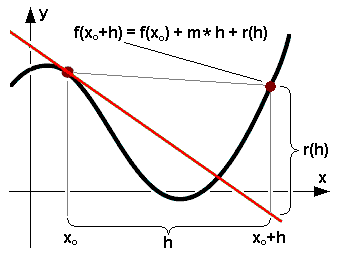
\includegraphics[width=0.4\textwidth]{pictures/diff-definition.png}\end{center} %70% der Textbreite%TODO: Bild selber machen
\end{*anmerkung}

\begin{*anmerkung}
	Neben der oben genannten Definition gibt es noch eine weitere Definition, die sich des Differentialquotienten bedient:
	\begin{align}
		f\text{ differentierbar in }x_0 \iff \lim\limits_{x\to x_0}\frac{f(x)-f(x_0)}{x-x_0}= \lim\limits_{h\to 0}\frac{f(x_0+h)-f(x_0)}{h}\text{ exisitiiert}\notag
	\end{align}
	Diese Definition lässt sich im Kontext komplexer oder mehrdimensionaler Funktionen nicht anwenden, zudem sind Beweise wegen des Quotienten leichter zu führen.
\end{*anmerkung}

\begin{*remark}
	Affin lineare Abbildung $\tilde{A}(x) := f(x_0) + f'(x_0)\cdot(x-x_0)$ approximiert die Funktion $f$ in der Nähe von $x_0$ und heißt \begriff{Linearisierung} von $f$ in $x_0$ (man nennt \propref{definition_ableitung} auch Approximation 1. Ordnung von $f$ in der Nähe von $x_0$).
\end{*remark}

\begin{proposition}
	\proplbl{definition_ableitung_proposition}
	Sei $f:D\subset K^n\to K^m$, $D$ offen. Dann: \\
	$f$ ist differenzierbar in $x_0\in D$ mit Ableitung $f'(x_0) \in L(K^n, K^m)$ \gls{gdw} eine der folgenden Bedingungen erfüllt ist:
	\begin{enumerate}[label={\alph*)},mode=unboxed]
		\item \label{satz_equivalenz_ableitungen_a} \itemEq{\proplbl{definition_ableitung_eins}f(x) &= f(x_0) + f'(x_0) \cdot (x-x_0) + r(x) \quad \forall x\in D}
		für ein $r: D\to K^m$ mit $\lim\limits_{\substack{x\to x_0 \\ x\neq x_0}} \frac{r(x)}{\vert x - x_0 \vert} = 0$
		\item \proplbl{satz_equivalenz_ableitungen_b} \itemEq{f(x) =f(x_0) + f'(x_0) \cdot (x-x_0) + R(x) (x-x_0)\quad\forall x\in D\proplbl{definition_ableitung_zwei}}
		für ein $R:D \to L(K^n, K^m)$ ($\cong K^{m\times n}$) mit $\lim\limits_{x\to x_0} R(x) = 0$ (d.h. Matrizen $R(x) \xrightarrow{x\to x_0}$ Nullmatrix in $K^{m\times n}$)
		\item \label{satz_equivalenz_ableitungen_c} \itemEq{\proplbl{definition_ableitung_drei}f(x) = f(x_0) + Q(x) (x - x_0) \quad \forall x\in D} für ein $Q:D\to L(K^n, K^m)$ ($\cong K^{m\times n}$) mit $\lim\limits_{x\to x_0} Q(x) = f'(x_0)$ (d.h. Matrizen $Q(x) \xrightarrow{x\to x_0}$ Matrix $f'(x_0)$ in $K^{m\times n}$)
	\end{enumerate}
\end{proposition}

\begin{*remark}
	Es gilt:
	\begin{align*}
	\text{\propref{definition_ableitung_eins}}\; \Leftrightarrow\; \lim\limits_{\substack{x\to x_0 \\ x\neq x_0}} \frac{f(x) - f(x_0) - f'(x_0) (x - x_0)}{\vert x - x_0 \vert} = 0
	\end{align*}
\end{*remark}

\begin{proof}
	\NoEndMark
	Aussage \ref{satz_equivalenz_ableitungen_a} ist leicht zu zeigen, anschließend erfolgt per Ringschluss die Äquivalenz der anderen Definitionen.
	\begin{enumerate}[label={zu \alph*)},leftmargin=\widthof{\ zu a)\ }]
		\item Offensichtlich ist $r(x) = o(\vert x - x_0 \vert ),$ $x\to x_0$ \\
		$\Rightarrow\;$ \ref{satz_equivalenz_ableitungen_a} $\Leftrightarrow$ $f$ ist differenzierbar in $x_0$ mit Ableitung $f'(x_0)$
	\end{enumerate}
	Ringschluss:
	\begin{itemize}[leftmargin=\widthof{\ a) $\rightarrow$ b):\ },topsep=-5pt]
		\item[a) $\Rightarrow$ b):] Sei $R: D\to K^{m\times n}$ gegeben durch \marginnote{$\otimes$: Tensorprodukt (siehe \cpageref{definition_tensorprodukt})}\begin{align*}
			R(x) &= \begin{cases}
				0, & x = x_0 \\
				\frac{r(x)}{\vert x - x_0\vert} \otimes (x - x_0)^T, & x\neq x_0
			\end{cases}\\
			\Rightarrow \;R(x) (x - x_0) &= \left( \frac{r(x)}{\vert x - x_0\vert^2} \otimes (x - x_0)^T \right) \cdot (x - x_0)\\
			 &= \frac{r(x)}{\vert x - x_0\vert ^2} \cdot \langle x - x_0 , x - x_0 \rangle = r(x) \quad \forall x\neq x_0
		\end{align*}
		Wegen $0 = r(x_0) = R(x_0)\cdot (x - x_0)$ folgt \begin{align*}
			\lim\limits_{x\to x_0} \vert R(x) \vert = \lim\limits_{\substack{x\to x_0 \\ x\neq x_0}} \frac{\vert r(x) \otimes (x - x_0)^T\vert }{\vert x - x_0 \vert^2} = \lim\limits_{\substack{x\to x_0 \\ x\neq x_0}} \frac{\vert r(x)\vert}{\vert x - x_0\vert} = 0
			\end{align*}
			
		\item[b) $\Rightarrow$ c):] Setzte $Q(x) := f'(x_0) + R(x) \; \forall x\in D$ $\Rightarrow$ \propref{definition_ableitung_drei}. Wegen $\lim\limits_{x\to x_0} Q(x) = f'(x_0)$ folgt \ref{satz_equivalenz_ableitungen_c}.
			
		\item[c) $\Rightarrow$ a):] Setzte $r(x) := (Q(x) - f'(x))\cdot (x - x_0) \;\forall x\in D$ $\Rightarrow$ \propref{definition_ableitung_eins}. Wegen $\vert r(x) \vert \le \vert Q(x) - f'(x_0) \vert \cdot \vert x - x_0 \vert $ folgt \zeroAmsmathAlignVSpaces \begin{align*}
			\lim\limits_{\substack{x\to x_0 \\ x\neq x_0}} \frac{\vert r(x) \vert}{\vert x - x_0 \vert} =  \lim\limits_{\substack{x\to x_0 \\ x\neq x_0}} \vert Q(x) - f'(x_0) \vert = 0
		\end{align*}
		\hfill$\square$
	\end{itemize}
\end{proof}

\begin{proposition}
	\proplbl{diffbar_impl_stetig}
	Sei $f:D\subset K^n \to K^m$, $D$ offen, differenzierbar in $x_0\in D$. Dann:
	\begin{enumerate}[label={\arabic*)}]
		\item $f$ ist stetig in $x_0$
		\item Die Ableitung $f'(x_0)$ ist eindeutig bestimmt.
	\end{enumerate}
\end{proposition}

\begin{proof}
	\begin{enumerate}
		\item Sei $A,\tilde{A}\in L(K^n,K^m)$ Ableitungen von $f$ in $x_0$, betrachte $x=x_0+ty$, wobei $y\in K^n$ mit $\vert y\vert =1$ fest, $t\in\real_{>0}$ (offenbar $\vert x-x_0\vert=t$) \\
		$\Rightarrow (A-\tilde{A})(ty)=o(\vert ty\vert)\Rightarrow (A-\tilde{A})(y)=\frac{o(t)}{t}\to 0$ \\
		$\Rightarrow (A-\tilde{A})(y)=0\Rightarrow A-\tilde{A}=0\Rightarrow A=\tilde{A}\beha$
		\item $\lim f(x)=1=\lim\big(f(x_0)+f'(x_0)(x-x_0)+o(\vert x-x_0\vert)\big)=f(x_0)\beha$
	\end{enumerate}
\end{proof}

\subsection{Spezialfälle für \texorpdfstring{$K=\mathbb{R}$}{K=R}}
\begin{enumerate}[label={\arabic*)},leftmargin=\widthof{1)\ },topsep=-5pt]
	\item \proplbl{spezialfall_ableitung_m1_item} \uline{$m=1\negthickspace:\, f\negthickspace:\mathbb{R}^n\to \mathbb{R}$}\\[0.6ex]
	$f'(x_0)\in \mathbb{R}^{1\times n}$ ist Zeilenvektor, $f'(x_0)$ betrachtet als Vektor im $\mathbb{R}^n$ auch \begriff{Gradient} genannt.
	
	Offenbar gilt $f'(x_0)\cdot y = \langle f'(x_0), y\rangle\;\forall y\in\mathbb{R}^n$ (Matrizenmultiplikation = Skalarprodukt) \\
	$\Rightarrow$ \propref{definition_ableitung_zwei} hat die Form \begin{align}
		\proplbl{spezialfall_ableitung_m1}
		f(x) = \underbrace{f(x_0) + \langle f'(x_0), x - x_0\rangle}_{\mathclap{\text{affin lineare Funktion: }\tilde{A}: \mathbb{R}\to \mathbb{R} \,(\text{in }x)}} + o\big( \vert x - x_0\vert \big)
	\end{align}
	Graph von $f$ ist Fläche im $\mathbb{R}^{n\times 1}$, genannt \begriff{Tangentialebene} vom Graphen von $f$ in $\big(x_0, f(x_0)\big)$.
	
	\item \proplbl{spezialfall_ableitung_n1} \uline{$n=1\negthickspace: f\negthickspace: D\subset \mathbb{R}\to \mathbb{R}^n$}\\[0.6ex]
	$f$ (bzw.  Bild $f[D]$) ist Kurve im $\mathbb{R}^n$ ($\cong \mathbb{R}^{m\times 1}$). \propref{definition_ableitung_zwei} kann man schreiben als \begin{align*}
		f(x_0 + t) = \underbrace{f(x_0) + t\cdot f'(x_0)}_{\mathclap{\text{Affin lineare Abb. }\tilde{A}:\mathbb{R}\to \mathbb{R}^m \text{ (in $t$)}}} + o(t), t\to 0, t\in\mathbb{R}
	\end{align*}
	\zeroAmsmathAlignVSpaces
	\begin{alignat}{2}
		\notag &\Leftrightarrow\quad& \underbrace{\frac{f(x_0 + t) - f(x_0)}{t}}_{\mathclap{\text{\begriff{Differenzenquotient} von $f$ in $x_0$}}} &= f'(x_0) + o(1), t\to 0 \\
		\proplbl{differentialquotient} &\Leftrightarrow& \underbrace{\lim\limits_{t\to 0} \frac{f(x_0 + t) - f(x_0)}{t}}_{\mathclap{\text{Differentialquotient}}} &= f(x_0)
	\end{alignat}
	
	\emph{beachte:} \begin{itemize}
		\item $f$  \gls{diffbar} in $x_0$ $\Leftrightarrow$ Differentialquotient existiert in $x_0$
		\item \propref{differentialquotient} nicht erklärt im Fall von $n>1$
	\end{itemize}

	\begin{interpretation}[ für $m > 1$]
		$f'(x_0)$ heißt \begriff{Tangentenvektor} an die Kurve in $f(x_0)$. Falls $f$ nicht  \gls{diffbar} in $x_0$ bzw. $x_0$ Randpunkt in $D$ und ist $f(x_0)$ definiert, so betrachtet man in \propref{differentialquotient} auch einseitige Grenzwerte (vgl. \propref{einseitige_grenzwerte}).
		
		$\lim\limits_{t\downarrow 0} \frac{f(x_0 + t) - f(x_0)}{t} = f_r'(x_0)$ heißt \begriff[Ableitung!]{rechtsseitige} \uline{Ableitung} von $f$ in $x_0$ (falls existent), analog ist $\lim\limits_{t\uparrow 0}$ die \begriff[Ableitung!]{linksseitige} \uline{Ableitung} $f_l'(x_0)$.
	\end{interpretation}

	\item \uline{$n=m=1\negthickspace:\;f\negthickspace: D\subset \mathbb{R}\to \mathbb{R}$} (vgl. Schule)\\[0.6ex]
	$f'(x_0)\in \mathbb{R}$ ist Zahl und \propref{differentialquotient} gilt (da Spezialfall von \propref{spezialfall_ableitung_n1}).
	
	\emph{Beobachtung:} \propref{spezialfall_ableitung_n1} gilt allgemein für $n=1$, nicht für $n>1$!
\end{enumerate}
\vspace*{1.5
	em}

\begin{conclusion}
	Sei $f:D\subset K\to K^n$, $D$ offen. Dann:
	\begin{align}
		\notag& \text{$f$ ist differenzierbar in $x_0\in D$ mit Ableitung $f'(x_0)\in L(K, K^m)$} \\
		\Leftrightarrow\quad
		& \proplbl{differentialquotient_prop} \exists f'(x_0) \in L(K, K^m): \lim\limits_{y\to 0} \frac{f(x_0 + y) - f(x_0)}{y} = f'(x_0) \\
		\notag 
		& \text{alternativ: } \lim\limits_{x\to x_0} \frac{f(x) - f(x_0)}{x - x_0} = f'(x_0)
	\end{align}
\end{conclusion}

\subsection{Einfache Beispiele für Ableitungen}
\begin{example}[affin lineare Funktionen]
	\proplbl{ableitung_linear}
	Sei $f:K^n\to K^m$ affin linear, d.h. \begin{align*}
		f(x) = A\cdot x + a\quad \forall x\in K^n, \text{ mit } A\in L(K^n, K^m), \, a\in K^m \text{ fest}
	\end{align*}
	Dann gilt für beliebiges $x_0\in K^n$:
	\zeroAmsmathAlignVSpaces**
	\begin{align*}
		f(x) &= A\cdot x_0 + a + A(x - x_0) \\
		&=f(x_0) + A(x - x_0)
	\end{align*}
	\zeroAmsmathAlignVSpaces
	\begin{align*}
		\xRightarrow{(\ref{definition_ableitung})}\;\; \text{$f$ ist  \gls{diffbar} in $x_0$ mit } f'(x_0) = A
	\end{align*}
	Insbesondere gilt für konstante Funktionen $f'(x_0) = 0$
	\begin{center}\begin{tikzpicture}
		\begin{axis}[
		xmin=-5, xmax=5, xlabel=$x$,
		ymin=-5, ymax=5, ylabel=$y$,
		samples=400,
		axis y line=middle,
		axis x line=middle,
		]
		\addplot+[mark=none] {2*x};
		\addlegendentry{$2x$}
		\addplot+[mark=none, dashed] {2};
		\addlegendentry{$2$}
		\end{axis}
		\end{tikzpicture}\end{center}
\end{example}

\begin{example}[quadratische Funktion]
	\proplbl{ableitung_beispiel_euklidische_norm}
	Sei $f:\real^n\to \real$ mit $f(x)=\vert x\vert^2$ \\
	für beliebiges $x_0$ gilt:
	\begin{align}
		\vert x-x_0\vert^2 &= \langle x-x_0,x-x_0\rangle \notag \\
		&= \vert x\vert^2 - \vert x_0\vert^2 - 2\langle x_0,x-x_0\rangle \notag
	\end{align}
	$\Rightarrow f(x) = f(x_0) + 2\langle \underbrace{2x_0}_{\text{Ableitung}},x-x_0\rangle + \underbrace{\vert x-x_0\vert^2}_{o(\vert x-x_0\vert)}$ \\
	$\Rightarrow f$ ist differenzierbar in $x_0$ mit $f'(x_0)=2x_0$, offenbar ist $f'$ stetig, also $f\in C^1(\real^n)$
 	\begin{center}\begin{tikzpicture}
 		\begin{axis}[
 		xmin=-5, xmax=5, xlabel=$x$,
 		ymin=-5, ymax=5, ylabel=$y$,
 		samples=400,
 		axis y line=middle,
 		axis x line=middle,
 		]
 		\addplot+[mark=none] {abs(x)^2};
 		\addlegendentry{$\vert x\vert^2$}
 		\addplot+[mark=none, dashed] {2*x};
 		\addlegendentry{$2x$}
 		\end{axis}
 		\end{tikzpicture}\end{center}
\end{example}

\begin{example}[Funktionen mit höherem Exponent]
	Sei $f:K\to K$, $f(x) = x^k$, $k\in\mathbb{N}$.
	\begin{itemize}[leftmargin=\widthof{$\,k=0$:\ }]
		\item[$k=0$:] $f(x) = 1\;\forall x$ $\Rightarrow$ $f'(x_0) = 0\;\forall x_0\in\mathbb{C}$ (vgl. \propref{ableitung_linear})
		\item[$k\ge 1$:] Es gilt \\
		\renewcommand{\arraystretch}{1.2}
		\begin{tabularx}{\linewidth}{r@{\ \ }r@{$\,$}X}
			& $(x_0 + y)^k$ & $\displaystyle = \sum_{j=0}^{k}\binom{k}{j} x_0^{k-j}\cdot y^j = x_0^k + k\cdot x_0^{k-1}\cdot y + o(y),\;y\to 0$ \\
			$\Rightarrow$ & $f(x_0 + y)$ & $= f(x_0) + k\cdot x_0^{k-1}\cdot y + o(y), y\to 0$ \\
			$\xRightarrow{(\ref{definition_ableitung})}$ & $f'(x_0)$ & $= k\cdot x_0^{k-1}$
		\end{tabularx}
	\end{itemize}
	\emph{beachte:} gilt in $\mathbb{C}$ und $\mathbb{R}$.
	\begin{center}\begin{tikzpicture}
		\begin{axis}[
		xmin=-5, xmax=5, xlabel=$x$,
		ymin=-5, ymax=5, ylabel=$y$,
		samples=400,
		axis y line=middle,
		axis x line=middle,
		]
		\addplot+[mark=none] {x^3};
		\addlegendentry{$x^3$}
		\addplot+[mark=none, dashed] {3*x^2};
		\addlegendentry{$3x^2$}
		\end{axis}
		\end{tikzpicture}\end{center}
\end{example}

\begin{example}[Exponentialfunktion]
	$f:K\to K$ mit $f(x)=e^x$ \\
	mit Differentialquotient $\Rightarrow$ $f$ ist differenzierbar mit $f'(x_0)=e^{x_0}\Rightarrow f\in C^1(K)$
	\begin{center}\begin{tikzpicture}
		\begin{axis}[
		xmin=-5, xmax=5, xlabel=$x$,
		ymin=-5, ymax=5, ylabel=$y$,
		samples=400,
		axis y line=middle,
		axis x line=middle,
		]
		\addplot+[mark=none] {e^x};
		\addlegendentry{$e^x$}
		\addplot+[mark=none, dashed] {e^x};
		\addlegendentry{$e^x$}
		\end{axis}
		\end{tikzpicture}\end{center}
\end{example}

\begin{example}[Betragsfunktion]
	\proplbl{ableitung_beispiel_betrag}
	$f:\real^n\to \real$ mit $f(x)=\vert x\vert$ \\
	$f$ ist nicht differenzierbar in $x_0=0$, denn angenommen, $f'(x_0)\in\real^n$ existiert und fixiere $y\in\real^n$, $\vert y\vert=1$ \\
	$\Rightarrow \vert ty\vert=0+\langle f'(0),ty\rangle + o(\vert t\vert)$, $t\to 0$ \\
	$\Rightarrow t\neq 0\Rightarrow \frac{\vert t\vert}{t}=\langle f'(0),y\rangle+\frac{o(t)}{t}\Rightarrow\pm 1 =$ feste Zahl in $\real_+\to 0\Rightarrow\lightning\beha$
	
	\emph{Folglich:} $f$ stetig in $x_0\not\Rightarrow f$ differenzierbar in $x_0$, das heißt Umkehrung von \propref{diffbar_impl_stetig} gilt nicht!
	
	\begin{hint}
		Es gibt stetige Funktion $f:\mathbb{R}\to \mathbb{R}$, die in keinem Punkt $x$ \gls{diffbar} ist (siehe Hildebrand, Analysis 1 S. 192 oder Königsberger Analysis 1, Kap. 9.11)
	\end{hint}

	\begin{center}\begin{tikzpicture}
		\begin{axis}[
		xmin=-5, xmax=5, xlabel=$x$,
		ymin=-5, ymax=5, ylabel=$y$,
		samples=400,
		axis y line=middle,
		axis x line=middle,
		]
		\addplot+[mark=none] {abs(x)};
		\addlegendentry{$\vert x \vert$}
		\end{axis}
	\end{tikzpicture}\end{center}
\end{example}

\begin{proposition}[Rechenregeln]
	\proplbl{ableitung_rechenregeln}
	Sei $D\in K^n$ offen, $f,g: D\to K^m$, $\lambda: D\to K$  \gls{diffbar} in $x_0\in D$ \\
	$\Rightarrow$ $(f\pm g): D\to K^m, (\lambda\cdot f):D\to K^m, (f\cdot g):D\to K$ sind  \gls{diffbar} in $x_0\in D$ und $\frac{1}{\lambda}:D\to K$ ist  \gls{diffbar} in $x_0$, falls $\lambda(x_0)\neq 0$
	mit
	\begin{enumerate}[label={\alph*)}]
		\item $(f\pm g)'(x_0) = f'(x_0) \pm g'(x_0)\in K^{m\times 1}$
		\item $(\lambda\cdot f)'(x_0) = \lambda (x_0)\cdot f'(x_0) + f(x_0)\cdot \lambda'(x_0)\in K^{m\times n}$
		\item $(f\cdot g)' (x_0) = \transpose{f(x_0)}\cdot g'(x_0) + \transpose{g(x_0)}\cdot f'(x_0)\in K^{m\times n}$
		\item $\left( \frac{\mu}{\lambda}\right)'(x_0) = \frac{\mu'(x_0)\cdot\lambda(x_0)-\mu(x_0)\cdot \lambda'(x_0)}{(\lambda(x_0))^2}$
	\end{enumerate}
\end{proposition}
\begin{proof}
	\begin{itemize}
		\item $f(x_0)\pm g(x_0)+(f'(x_0))(x-x_0)\pm (g'(x_0))(x-x_0)+o(\vert x-x_0\vert) =f(x_0)\pm g(x_0)+\big(f'(x_0)\pm g'(x_0)\big)(x-x_0)+o(\vert x-x_0\vert)\beha$
		\item $\lambda(x)f(x)=\big(\lambda(x_0)+\lambda'(x_0)(x-x_0)+o(\vert x-x_0\vert)\big)\cdot\big(f(x_0)+f'(x_0)(x-x_0)+o(\vert x-x_=\vert)\big) = \lambda(x_0)f(x_0) - \big(\lambda'(x_0)f(x_0)+\lambda(x_0)f'(x_0)\big)(x-x_0)+o(\vert x-x_0\vert)\beha$
		\item analog
		\item zeige $\left(\frac{1}{\lambda}\right)'(x_0)=-\frac{\lambda'(x_0)}{\lambda(x_0)^2}$, Rest folgt mit $f=\mu$ \\
		$\frac{1}{\lambda(x)}-\frac{1}{\lambda(x_0)}=\frac{\lambda(x_0)-\lambda(x)}{\lambda(x)\lambda(x_0)} = ... = \left(\frac{-\lambda'(x_0)}{\lambda(x_0)^2}\right)(x-x_0)+o(\vert x-x_0\vert)\beha$
	\end{itemize}
\end{proof}

\begin{example}
	Sei $f:D\in K^n\to K^m$, $c\in K$, $f$  \gls{diffbar} in $x_0\in D$\\
	$\xRightarrow{\ref{ableitung_rechenregeln}\ b)} (c\cdot f) = c\cdot f'(x_0)$ (da $c$ konst. Funktion $D\to K$)
\end{example}

\begin{example}[Polynom]
	Sei $f:K\to K$, Polynom $f(x) = \sum\limits_{l=0}^{k}a_l x^l$ \\
	$\Rightarrow$ $f$  \gls{diffbar} $\forall x_0\in K$ mit $f'(x_0) = \sum\limits_{l=1}^k l a_l x_0^{l-1}$
\end{example}

\begin{example}
	Sei $f=\frac{f_1}{f_2}$ rationale Funktion auf $\mathbb{R}$ (d.h. $f_1, f_2:K\to K$ Polynom) \\
	$\Rightarrow$ $f$ ist  \gls{diffbar} auf $K\setminus \{ \text{Nullstellen von }f_2 \}$
\end{example}

\begin{example}[Sinus und Cosinus]
	$\sin, \cos: K\to K$ ($\mathbb{R}$ bzw. $\mathbb{C}$) $\forall x_0\in K$.
	
	Denn:{\zeroAmsmathAlignVSpaces
	\begin{align*}
		 \frac{\sin y}{y} = \frac{e^{iy} - e^{-iy}}{2iy} = \frac{1}{2}\cdot \left( \frac{e^{iy} - 1}{iy} + \frac{e^{-iy} - 1}{-iy} \right) \xrightarrow[\text{vgl. \eqref{exp_limit_1}}]{y\to 0} 1,
	\end{align*}}
	folglich {\zeroAmsmathAlignVSpaces*
	\begin{align*}
		\lim\limits_{y\to 0} \frac{\sin(x_0 + y) - \sin(x_0)}{y} &\overset{\star}{=} \lim\limits_{y\to 0} \frac{2}{y} \cos\left( x_0 + \frac{y}{2}\right) \cdot \sin \left( \frac{y}{2}\right) \marginnote{$\star$: Additionstheoreme} \\
		&= \lim\limits_{y\to 0} \frac{2}{y}\cdot\sin\left(\frac{y}{2}\right)\cdot\cos\left(x_0 + \frac{y}{2}\right)\\
		&= \cos x_0 \quad\forall x_0\in K
		\end{align*}}
		
	Analog für den Kosinus.
	
	\begin{center}\begin{tikzpicture}
		\begin{axis}[
		xmin=-5, xmax=5, xlabel=$x$,
		ymin=-5, ymax=5, ylabel=$y$,
		samples=400,
		axis y line=middle,
		axis x line=middle,
		]
		\addplot+[mark=none] {sin(deg(x))};
		\addlegendentry{$\sin(x)$}
		\addplot+[mark=none, dashed] {cos(deg(x))};
		\addlegendentry{$\cos(x)$}
		\end{axis}
		\end{tikzpicture}
		\begin{tikzpicture}
		\begin{axis}[
		xmin=-5, xmax=5, xlabel=$x$,
		ymin=-5, ymax=5, ylabel=$y$,
		samples=400,
		axis y line=middle,
		axis x line=middle,
		]
		\addplot+[mark=none] {cos(deg(x))};
		\addlegendentry{$\cos(x)$}
		\addplot+[mark=none, dashed] {- sin(deg(x))};
		\addlegendentry{$-\sin(x)$}
		\end{axis}
		\end{tikzpicture}\end{center}
\end{example}

\subsection{Rechenregeln}
\begin{*definition}
	Sei $f:D\subset K^n \to K^m$, $D$ offen.
	
	Falls $f$  \gls{diffbar} in allen $x_0\in D$, dann heißt $f$ \begriff{differenzierbar} auf $D$ und Funktion $f':D\to L(K^n, K^m)$ heißt \begriff{Ableitung} von $f$.
	
	Ist zusätzlich Funktion $f': D\to L(K^n, K^m)$ stetig, dann heißt Funktion $f$ \begriff{stetig differenzierbar} (auf $D$) bzw. \mathsymbol{C1}{$C^1$}\emph{-Funktion} (auf $D$).
	
	$C^1(D, K^m):= \left\lbrace f: D\to K^m \mid f \text{ stetig  \gls{diffbar} auf } D \right\rbrace$
\end{*definition}

\begin{example}
	\begin{enumerate}[label={\alph*)}]
		\item $f(x) = x^k\;\forall x\in\mathbb{R},\, k\in\mathbb{N}_{\ge 0}$ \\
		$\Rightarrow$ $f'(x) = k\cdot x^{k-1}\;\forall x\in \mathbb{R}$ \\
		$\Rightarrow$ offenbar stetige Funktion \\ $\Rightarrow$ $f\in C^1(\mathbb{R}, \mathbb{R})$
		
		\item $f(x) = e^x\;\forall x\in\mathbb{C}$ \\
		$\Rightarrow f'(x) = e^x \;\forall x\in\mathbb{C}$ stetig \\
		$\Rightarrow$ $f\in C^1(\mathbb{C},\mathbb{C})$
		
		\item $f(x) = \vert x \vert^2\;\forall x\in\mathbb{R}^n$ \\
		$\Rightarrow$ $f(x) = 2x\;\forall x\in\mathbb{R}^n$, offenbar stetig \\
		$\Rightarrow$ $f\in C^1(\mathbb{R}^n, \mathbb{R})$
	\end{enumerate}
\end{example}

\begin{example}
	\proplbl{ableitung_beipsiel_unstetige_ableitung}
	Sei $f:\mathbb{R}\to \mathbb{R}$ mit $f(0) = 0$, $f(x)=x^2\cdot \sin\left(\frac{1}{x}\right)$ $\forall x\neq 0$.
	
	\begin{center}\begin{tikzpicture}
		\begin{axis}[
		xmin=-5, xmax=5, xlabel=$x$,
		ymin=-5, ymax=5, ylabel=$y$,
		samples=400,
		axis y line=middle,
		axis x line=middle,
		]
		\addplot+[mark=none] {x^2*sin(deg(1/x))};
		\addlegendentry{$x^2\cdot \sin(\frac{1}{x})$}
		\end{axis}
		\end{tikzpicture}\end{center}
	
	Wegen \begin{align*}
		\frac{\vert x^2 \cdot \sin \frac{1}{x}\vert}{\vert x \vert} \le \vert x \vert \xrightarrow{x\neq 0} 0
	\end{align*}
	folgt{ \zeroAmsmathAlignVSpaces \begin{align*}
		& f(x) = o(\vert x \vert), x\to 0 \\
		\Rightarrow\;& f(x) = f(0) + 0\cdot (x - 0) + o(\vert x - 0\vert), x\to 0 \\
		\Rightarrow\;& f \text{  \gls{diffbar} in $x=0$ mit $f'(0) = 0$}
	\end{align*}}
	
	Rechenregeln liefern $x\neq 0$: \begin{align*}
		f'(x) = 2x\cdot\sin\frac{1}{x}- \cos\frac{1}{x} \quad\forall x\neq 0
	\end{align*}
	
	Für $x_k := \frac{1}{k\pi}$ gilt: \begin{align*}
		& \lim\limits_{k\to\infty} 2 x_k \cdot \sin \frac{1}{x_k} = 0,\; \lim\limits_{k\to\infty} \cos \frac{1}{x_k} = \pm 1 \\
		\Rightarrow\;& \lim\limits_{x\to 0} f'(x) \text{ existiert nicht} \\
		\Rightarrow\;& f\notin C^1(\mathbb{R}, \mathbb{R}),
	\end{align*}
	d.h. Ableitung einer stetigen Funktion muss \emph{nicht} stetig sein.
\end{example}

\begin{boldenvironment}[Man beobachtet]
	\hspace{0pt}
\begin{itemize}[topsep=-2pt]
	\item \propref{definition_ableitung} bzw. \propref{definition_ableitung_zwei_stern} sind häufig ungeeignet zum Bestimmen von $f'(x_0)$
	\item \propref{differentialquotient_prop} ist durchaus nützlich für konkrete Fälle im Fall $n=1$
	
	\emph{$\rightarrow$ Strategie:} Zurückführung auf einfachere Fälle durch Rechenregeln und Reduktion
\end{itemize}
\end{boldenvironment}



\begin{conclusion}
	\proplbl{ableitung_quotientenregel}
	Seien $\lambda$, $\mu:D\to K$  \gls{diffbar} in $x_0$, $D$ offen und $\lambda(x_0)\neq 0$ \\
	$\Rightarrow$ $\left( \frac{\mu}{\lambda} \right): D\to K$  \gls{diffbar} in $x_0$ mit \begin{align*}
		\left( \frac{\mu}{\lambda} \right)' (x_0) = \frac{\lambda(x_0)\cdot \mu'(x_0) - \mu(x_0) \cdot \lambda'(x_0)}{\lambda(x_0)^2}\in K^{1\times n}
	\end{align*}
\end{conclusion}

\begin{proof}[\propref{ableitung_quotientenregel}]
	Setzte in \propref{ableitung_rechenregeln} $f=\mu$ (d.h. $m=1$) und betr. Produkt $\frac{1}{\lambda}\cdot \mu$.
\end{proof}

\begin{proposition}[Kettenregel]
	\proplbl{ableitung_kettenregel}
	Sei $f:D\subset K^n\to K^m$, $g:\tilde{D}\subset K^m\to K^l$, $D$,$\tilde{D}$ offen, $f$  \gls{diffbar} in $x_0\in D$, $g$  \gls{diffbar} in $f(x_0)\in\tilde{D}$ \\
	$\Rightarrow$ $g\circ f: D\to K^l$  \gls{diffbar} in $x_0$ mit $(g\circ f)' = g'(f(x))\cdot f'(x)$ ($\in K^{l\times n}$)
\end{proposition}
\begin{proof}
	\begin{align}
		(g\circ f)(x)  = g(f(x)) &= g(f(x_0)) + g'(f(x_0))(f(x)-f(x_0)) + o(\vert f(x)-f(x_0)\vert) \notag \\
		&= (g\circ f)(x_0) + g'(f(x_0))\cdot f(x_0)(x-x_0) + o(\vert x-x_0\vert)
	\end{align}
	$\Rightarrow$ Behauptung
\end{proof}

\begin{example}[$x$ im Exponenten]
	\proplbl{ableitung_beispiel_exponentialfunktion}
	$f:\mathbb{R}\to \mathbb{R}$, $f(x) = a^x$ ($a\in\mathbb{R}_{\ge 0}$, $a\neq 1$).
	Offenbar $a^x = \left(e^{\ln a}\right)^x = e^{x\cdot \ln a}$\\
	$\Rightarrow$ $f(x) = g(h(x))$ mit $g(y) = e^y$, $h(x) = x\cdot \ln a$
	$\Rightarrow g'(y)=e^y$, $h'(x)=\ln a\Rightarrow f'(x)=e^{x\cdot \ln a}\cdot \ln a=a^x\cdot\ln a$
	\begin{center}\begin{tikzpicture}
		\begin{axis}[
		xmin=-5, xmax=5, xlabel=$x$,
		ymin=-5, ymax=5, ylabel=$y$,
		samples=400,
		axis y line=middle,
		axis x line=middle,
		]
		\addplot+[mark=none] {2^x};
		\addlegendentry{$2^x$}
		\addplot+[mark=none, dashed] {2^x*ln(2)};
		\addlegendentry{$2^x\cdot \ln(2)$}
		\end{axis}
		\end{tikzpicture}\end{center}
\end{example}

\begin{example}[Logarithmus]
	\proplbl{ableitung_beispiel_logarithmus}
	$f:\real_{>0}\to \real$ mit $f(x)=\log_a x$, $a\in\real_{>0}$ und $a\neq 1$, $x_0\in \real_{>0}$ \\
	mit $y=\log_a x$, $y_0=\log_a x_0$ ist $x-x_0=a^y-a^{y_0}$ \\
	Differentialquotient $\Rightarrow f'(x)=\frac{1}{x\cdot\ln a}$, also $f\in C^1(\real_{>0})$
	
	Spezialfall: $(\ln(x))' = \frac{1}{x}$ $\forall x>0$
	\begin{center}\begin{tikzpicture}
		\begin{axis}[
		xmin=-5, xmax=5, xlabel=$x$,
		ymin=-5, ymax=5, ylabel=$y$,
		samples=400,
		axis y line=middle,
		axis x line=middle,
		]
		\addplot+[mark=none] {log2(x)};
		\addlegendentry{$\log_2(x)$}
		\addplot+[mark=none, dashed] {1/(x*ln(2))};
		\addlegendentry{$\frac{1}{x\cdot\ln(2)}$}
		\end{axis}
		\end{tikzpicture}\end{center}
\end{example}

\begin{example}
	Sei $f:\mathbb{R}_{>0}\to \mathbb{R}$, $f(x) = x^r$ ($r\in\mathbb{R}$)
	
	Wegen $x^r = e^{r\cdot \ln x}$ liefert Kettenregeln (analog zu \propref{ableitung_beispiel_exponentialfunktion}) \begin{align*}
	f'(x_0) = \frac{r\cdot e^{r\cdot \ln x_0}}{x_0} = \frac{r\cdot x_0^r}{x_0} = r\cdot x_0^{r - 1} \quad\forall x_0>0
	\end{align*}
	
	Spezialfall: $f(x) = \frac{1}{x^k}$ $\Rightarrow$ $f'(x) = - \frac{k}{x^{k+1}}$
	
	Zu \propref{ableitung_beipsiel_unstetige_ableitung}:\begin{align*}
	f'(x) = 2x\cdot \sin\frac{1}{x} + x^2\cdot \cos\frac{1}{x} \cdot \left( - \frac{1}{x^2}\right) = 2x\cdot \sin\frac{1}{x} - \cos\frac{1}{x}
	\end{align*}
\end{example}

\begin{example}[Tangens und Cotangens]
	\proplbl{ableitung_beispiel_tangens}
	$\tan: K\setminus \{ \frac{\pi}{2} + k\cdot \pi \mid k\in\mathbb{Z} \}\to K$, $\cot:K\setminus \{ k\cdot \pi \mid k\in\mathbb{Z} \} \to K$ \\[\dimexpr - \baselineskip / 2 \relax]
	\zeroAmsmathAlignVSpaces \begin{alignat*}{3}
	\xRightarrow{\text{Quotientenregel}}&\;\;& \tan'(x_0)&= \frac{\sin'(x_0)\cos (x_0) - \cos (x_0) \cdot \sin(x_0)}{\left( \cos(x_0)\right)^2} &&\\
	&& &= \frac{\cos^2(x_0) + \sin^2(x_0)}{\cos^2(x_0)} = \frac{1}{\cos^2(x_0)} && \forall x_0\in \text{ Definitionsbereich} \\
	&& \cot'(x_0) &= - \frac{1}{\sin^2(x_0)}&&\forall x_0\in\text{ Definitionsbereich}
	\end{alignat*}
	\begin{center}\begin{tikzpicture}
		\begin{axis}[
		xmin=-5, xmax=5, xlabel=$x$,
		ymin=-5, ymax=5, ylabel=$y$,
		samples=400,
		axis y line=middle,
		axis x line=middle,
		restrict y to domain=-5:5
		]
		\addplot+[mark=none] {tan(deg(x))};
		\addlegendentry{$\tan(x)$}
		\addplot+[mark=none, dashed] {1/(cos(deg(x)))^2};
		\addlegendentry{$\frac{1}{\cos^2(x)}$}
		\end{axis}
		\end{tikzpicture}
		\begin{tikzpicture}
		\begin{axis}[
		xmin=-5, xmax=5, xlabel=$x$,
		ymin=-5, ymax=5, ylabel=$y$,
		samples=400,
		axis y line=middle,
		axis x line=middle,
		restrict y to domain=-5:5
		]
		\addplot+[mark=none] {cot(deg(x))};
		\addlegendentry{$\cot(x)$}
		\addplot+[mark=none, dashed] {-1/(sin(deg(x))^2)};
		\addlegendentry{$-\frac{1}{\sin^2(x)}$}
		\end{axis}
		\end{tikzpicture}\end{center}
\end{example}





\begin{proposition}[Reduktion auf skalare Funktionen]
	\proplbl{ableitung_proposition_reduktion}
	Sei $f=(f_1, \dotsc, f_m): D\subset K^n\to K^m$, $D$ offen, $x_0\in D$. Dann gilt:\begin{center}
		$f$  \gls{diffbar} in $x_0$ $\Leftrightarrow$ alle $f_j$  \gls{diffbar} in $x_0$ $\forall j=1,\dotsc,m$
	\end{center}

	Im Fall der Differenzierbarkeit hat man: \begin{align}
		\proplbl{ableitung_jacobimatrix}
		f'(x_0) = \begin{pmatrix}
			f_1'(x_0) \\
			\vdots \\
			f_m'(x_0)
		\end{pmatrix} \in K^{m\times n}
	\end{align}
\end{proposition}
\smiley{} Wenn Sie das nächste mal aus der Disko kommen, zuviel getrunken haben und den Namen 
ihrer Freundin nicht mehr kennen, sollten sie sich daran aber noch erinnern: \smiley{} \\

\begin{remark}
	Mit \propref{ableitung_proposition_reduktion} kann man die Berechnungen der Ableitungen stets auf skalare Funktionen $f:D\subset K^n\to K$ zurückführen. Die Matrix in \propref{ableitung_jacobimatrix} besteht aus $m$ Zeilen $f_j'(x_0)\in K^{1\times m}$.
\end{remark}

\begin{example}
	Sei $f:\mathbb{R}\to \mathbb{R}^2$ mit \begin{align*}
		f(t) &= \begin{pmatrix}
			t\cdot \cos( 2\pi t) \\ t\cdot \sin(2\pi t)
		\end{pmatrix}, & f'(t) &= \begin{pmatrix}
			\cos(2\pi t) - t\cdot \sin(2\pi t)\cdot 2\pi \\ \sin(2\pi t)+ t\cdot\cos(2\pi t)\cdot 2\pi
		\end{pmatrix} \in \mathbb{R}^{2\times 1},
	\end{align*}
	und $f'(0) = \binom{1}{0}$, $f'(1) = \binom{1}{2\pi}$.
\end{example}

\begin{lemma}
	\proplbl{ableitung_spezialfall_reduktion_proposition}
	Sei $f=(f_1, f_2):D\subset K^n\to K^k\times K^l$, $D$ offen, $x_0\in D$.
	
	Funktion $f$ ist  \gls{diffbar} in $x_0$ genau dann, wenn $f_1:D\to K^k$ und $f_2 :D\to K^l$  \gls{diffbar} in $x_0$.
	
	Im Falle der Differenzierbarkeit gilt\begin{align}
		\proplbl{ableitung_spezialfall_reduktion}
		f'(x_0) = \begin{pmatrix}
			f_1'(x_0) \\ f_2'(x_0)
		\end{pmatrix} \in K^{(k+l)\times n}
	\end{align}
	
	\begin{hint}
		Da $K^k\times K^l$ mit $K^{k+l}$ identifiziert werden kann, kann man $f$ auch als Abbildung von $D$ nach $K^{k+l}$ ansehen. Dementsprechend kann die Matrix in \propref{ableitung_spezialfall_reduktion} der Form \begin{align*}
			\begin{pmatrix}
				(k\times n) \text{ Matrix} \\
				(l\times n) \text{ Matrix}
			\end{pmatrix}
		\end{align*}
		auch als $((k+l)\times n)$-Matrix aufgefasst werden.
	\end{hint}
\end{lemma}

\begin{proof}\hspace*{0pt}
	\NoEndMark
	\begin{itemize}[topsep=\dimexpr - \baselineskip / 3\relax]
		\item["`$\Rightarrow$"'] Man hat
		\zeroAmsmathAlignVSpaces[3pt][3pt]
		\begin{alignat}{2}
				\proplbl{ableitung_beweis_lemma_spezialfall_reduktion} && f(x) &= f(x_0) + f'(x_0)\cdot(x - x_0) + R(x)\cdot (x - x_0), \, \;R(x) \xrightarrow{x\to x_0}0
			\intertext{da $f'(x_0)$, $R(x)\in L(K^n, K^k\times K^l)$}
				\notag\Rightarrow&\;\;& f'(x_0) &= (A_1, A_2), \; R(x) = \big( R_1(x), R_2(x) \big))
			\intertext{mit $A_1, R_1(x)\in L(K^n, K^k)$, $A_2, R(x)\in L(K^n, K^l)$}
				\proplbl{ableitung_beweis_lemma_spezialfall_reduktion_einzelableitung} \xRightarrow{\eqref{ableitung_beweis_lemma_spezialfall_reduktion}}&& f_j(x)&= f_j(x_0) + A_j \cdot (x - x_0) + R_j(x) (x - x_0),\;R_j(x)\xrightarrow{x\to x_0}0 \\
				\notag\Rightarrow&& f_j & \text{ ist  \gls{diffbar} in $x_0$ mit $f_j'(x_0) = A_j$, $j=1,2$}
		\end{alignat}
		$\Rightarrow$ Behauptung
		\item["`$\Leftarrow$"'] (es gilt auch \eqref{ableitung_beweis_lemma_spezialfall_reduktion_einzelableitung} mit $A_j = f_j'(x_0)$)
		
		Setzte \begin{align*}
		 &A=\begin{pmatrix}
			f_1'(x) \\ f_2'(x)
		\end{pmatrix},\; R(x) = \begin{pmatrix}
			R_1(x) \\ R_2(x)
		\end{pmatrix} \\
		\xRightarrow{\eqref{ableitung_beweis_lemma_spezialfall_reduktion_einzelableitung}}\;& A, R(x)\in L(K^n, K^k\times K^l) \\
		\xRightarrow{\text{mit }A_j=f_j'(x_0)}\; & f(x)= f(x_0) + A(x - x_0) + R(x)(x - x_0), R(x)\xrightarrow{x\to x_0}0
		\end{align*}
		$\Rightarrow$ $f$  \gls{diffbar} in $x_0$ und \eqref{ableitung_spezialfall_reduktion} gilt.\hfill\csname\InTheoType Symbol\endcsname
	\end{itemize}
\end{proof}

\begin{proof}[\propref{ableitung_proposition_reduktion}]
	Mehrfache Anwendung von \propref{ableitung_spezialfall_reduktion_proposition} (z.B. mit $k=1, l = m - j$ für $j=1,\dotsc, m-1$)
\end{proof}
Integration kann betrachtet werden als
\begin{itemize}
	\item verallgemeinerte Summation, d.h. $\int_\mu f\D x$ ist Grenzwert von Summen
	\item lineare Abbildung $\int: \mathcal{F}\marginnote{$\mathcal{F}$: Menge der Funktionen}\to \mathbb{R}$ über $\int_a^b (\alpha f + \beta g)\D x = \alpha \int_a^b f \D x + \beta \int_a^b g \D x$ Funktionen, d.h. als Grundlage benötigt man ein "`Volumen"' (Maß) für allgemeine Mengen $M\subset\mathbb{R}$.
	
	Wir betrachten Funktionen $f:D\subset\mathbb{R}^n\to \mathbb{R}\cup \{ \pm \infty \}$, welche komponentenweise auf $f:D\subset\mathbb{R}\to K^k$ erweitert werden kann. Benutze $C^m \cong \mathbb{R}^{2m}$ für $K=\mathbb{C}$.
	
	Vgl. Buch:  Evans, Lawrence C.; Gariepy, Ronald F.: Measure theory and fine properties of functions
\end{itemize}
\include{./TeX_files/Differentiation_2}


\end{document}
